\section{Idee Iniziali di Progetto}

In questa sezione vengono presentati gli sketch iniziali di navigazione per i quattro Use Case identificati. Gli schemi sono stati progettati per mettere al centro l'esperienza utente, integrando nativamente le logiche di Realtà Aumentata e Gamification.

\subsection{UC1: Pianificazione e gestione del percorso}
In questa prima fase, l'utente interagisce con i punti di ingresso fisici (RFID) per avviare il tour. L'interfaccia guida il visitatore nella scelta del percorso più adatto alle proprie esigenze (tempo a disposizione, livello di approfondimento, accessibilità).

\begin{figure}[H]
    \centering
    \textbf{Use Case 1 - Versione 1} \\[0.5em]
    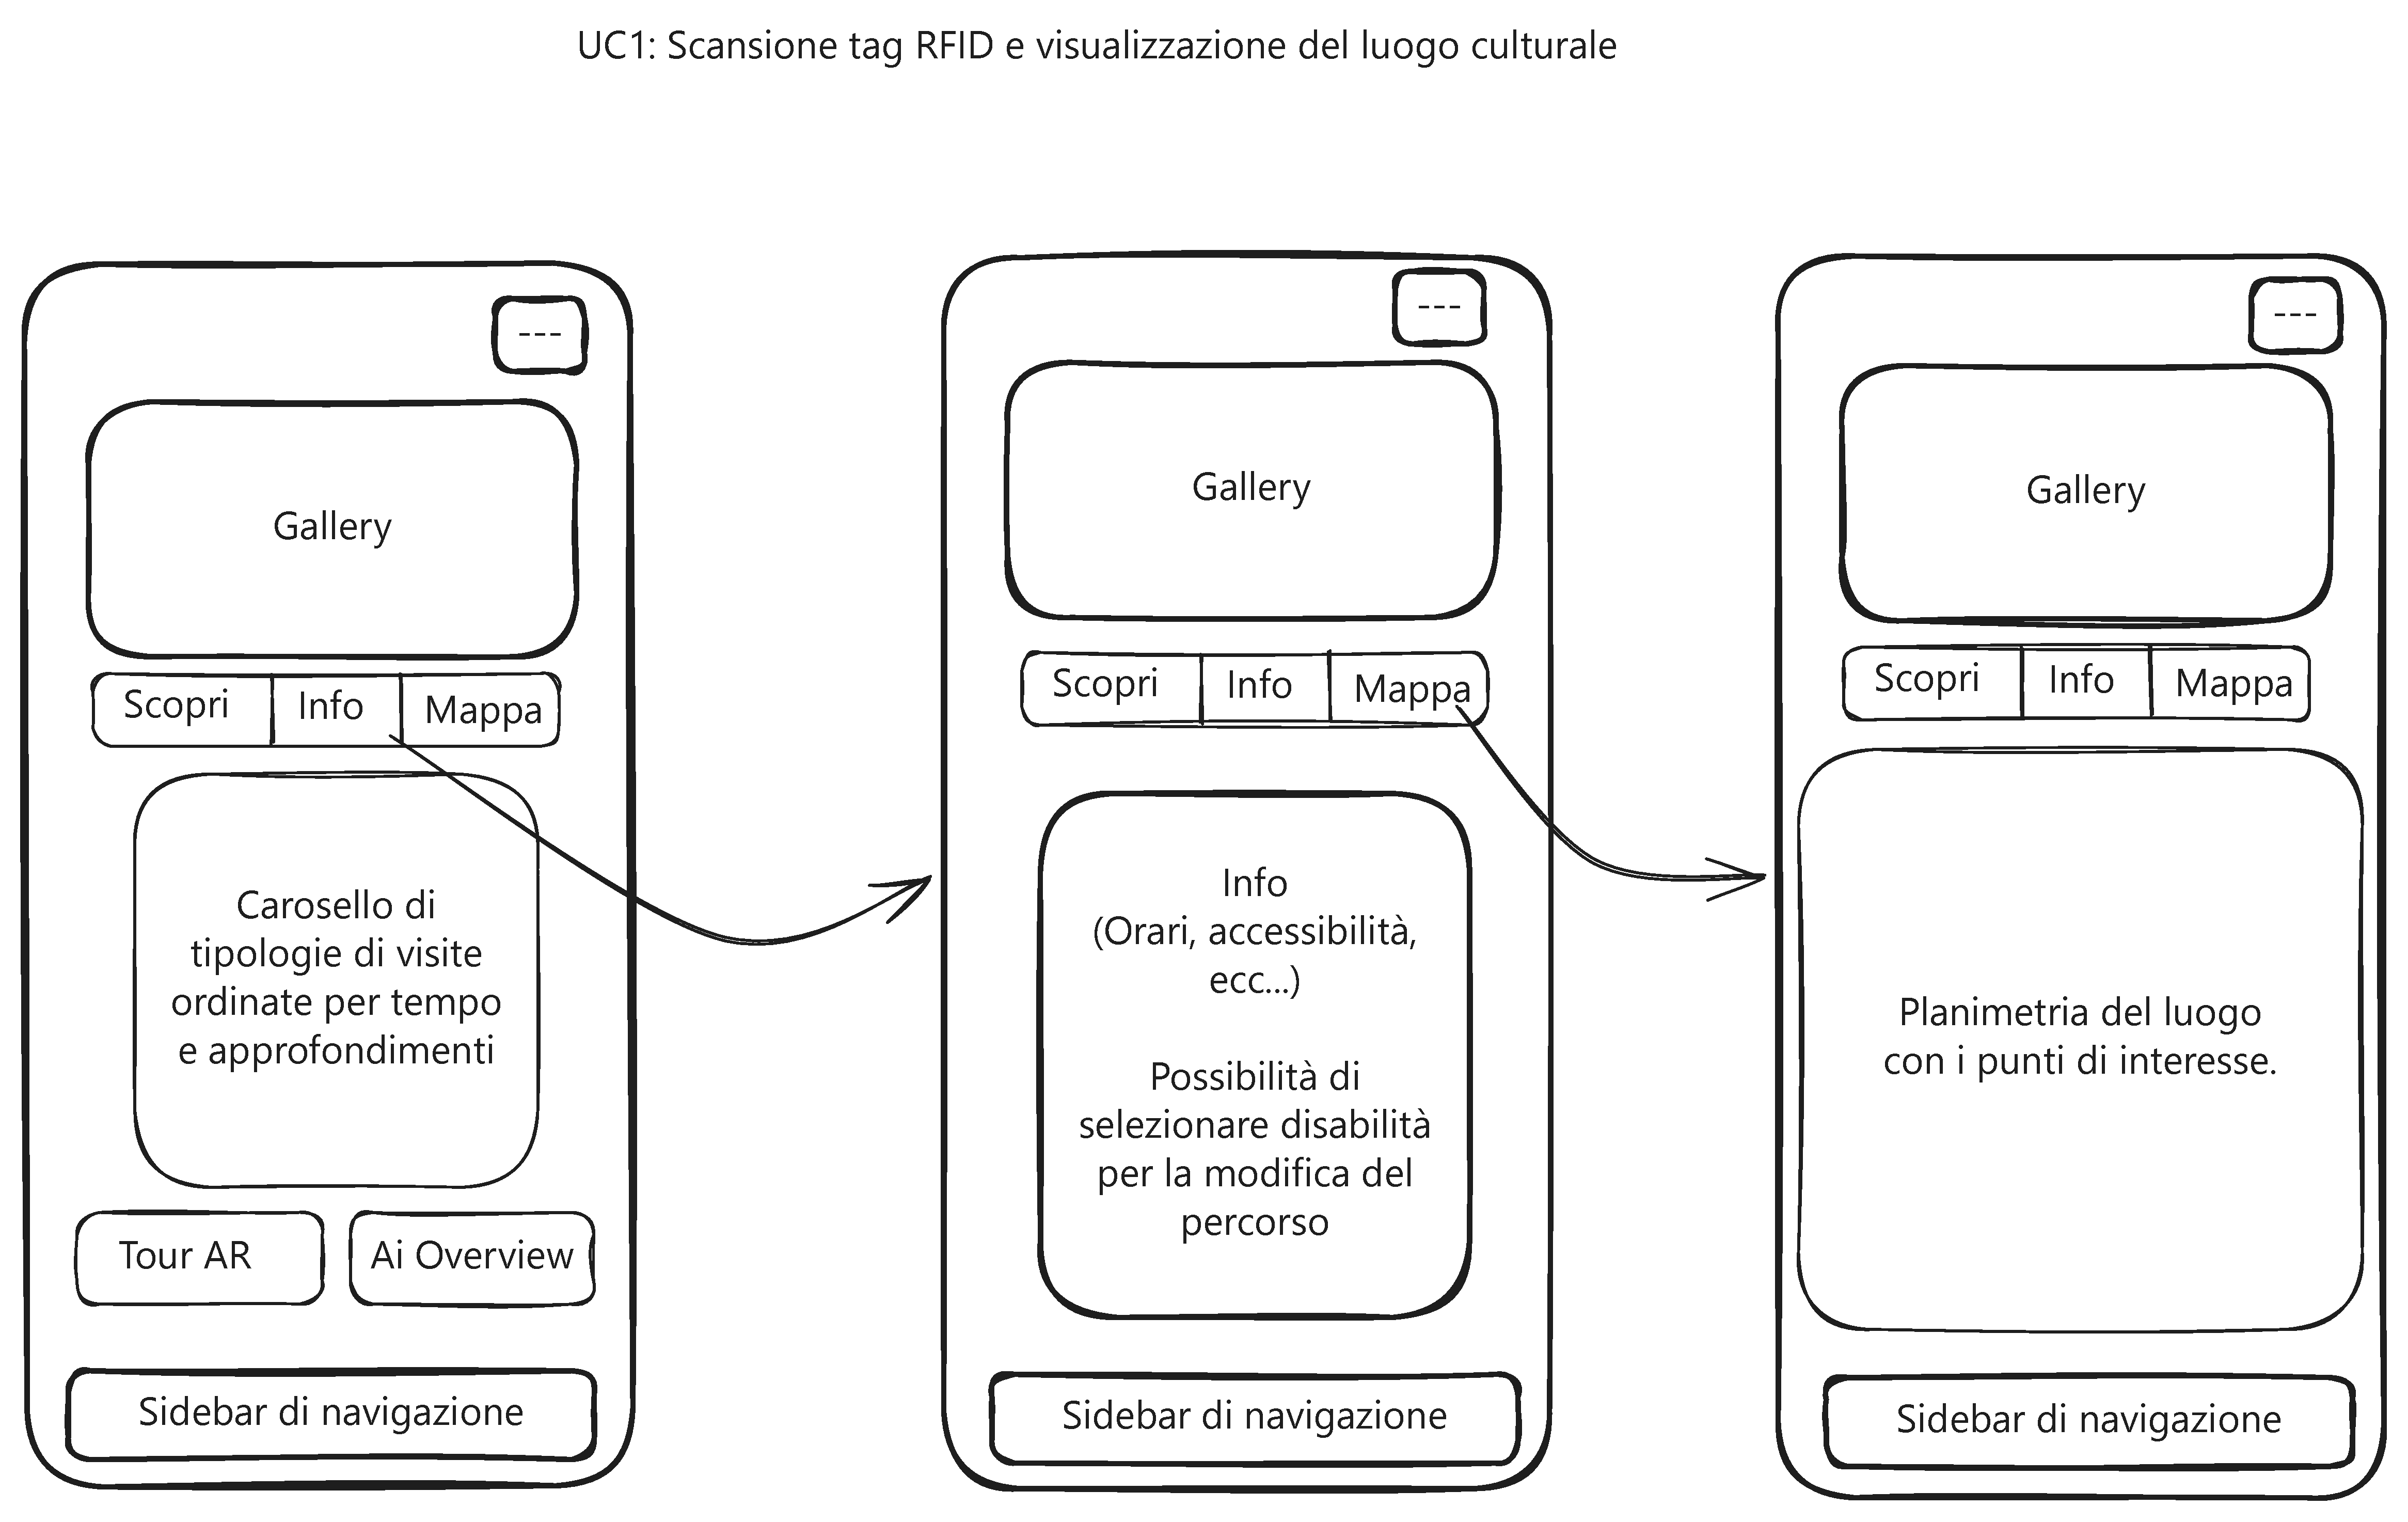
\includegraphics[width=0.9\textwidth,height=0.38\textheight,keepaspectratio]{../../../allegati/sketches/UC1_V1.pdf}
    \caption{Per consultare il PDF originale clicca \href{https://github.com/AntonioWalter/Culturia_IUM/blob/main/docs/allegati/sketches/UC1_V1.pdf}{[QUI]}}
    \label{fig:uc1_v1}
\end{figure}

\begin{figure}[H]
    \centering
    \textbf{Use Case 1 - Versione 2} \\[0.5em]
    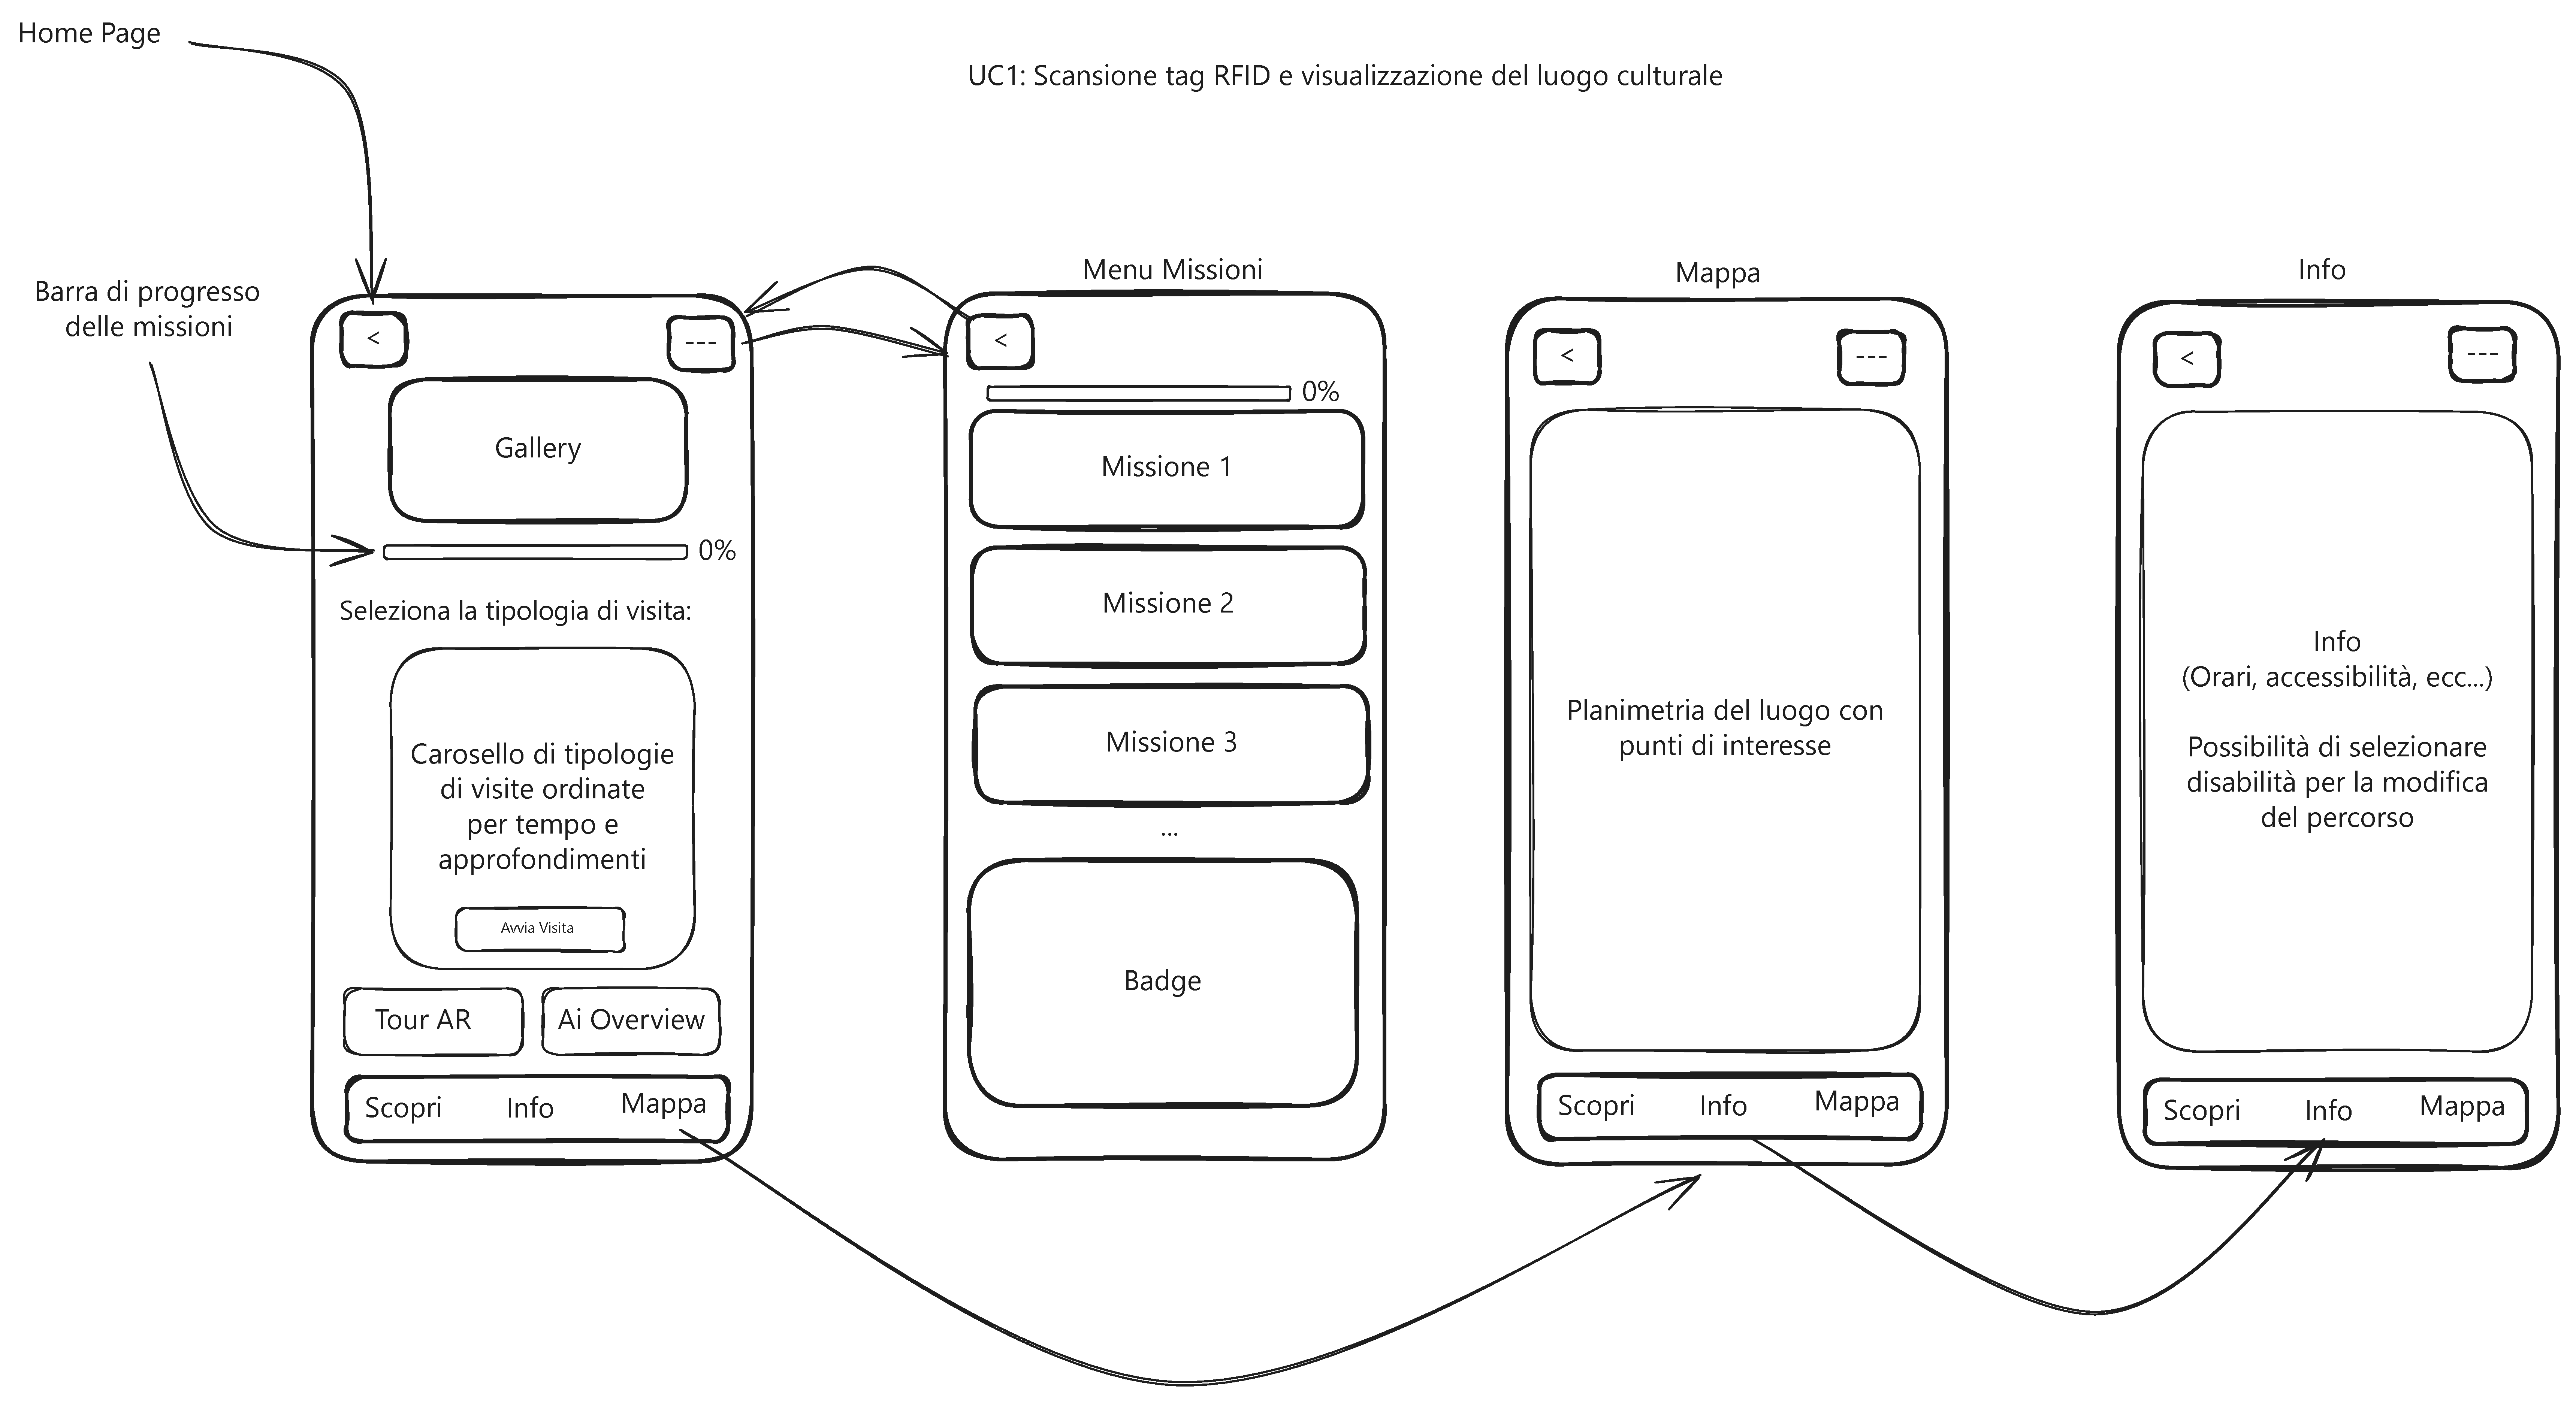
\includegraphics[width=0.9\textwidth,height=0.38\textheight,keepaspectratio]{../../../allegati/sketches/UC1_V2.pdf}
    \caption{Per consultare il PDF originale clicca \href{https://github.com/AntonioWalter/Culturia_IUM/blob/main/docs/allegati/sketches/UC1_V2.pdf}{[QUI]}}
    \label{fig:uc1_v2}
\end{figure}

\newpage
\subsection{UC2: Comprensione del patrimonio e approfondimento}
L'interfaccia si trasforma in una "lente attiva" tramite l'AR. L'obiettivo è abbattere le barriere informative fornendo contenuti stratificati tramite la mediazione dell'Intelligenza Artificiale.

\begin{figure}[H]
    \centering
    \textbf{Use Case 2 - Versione 1} \\[0.5em]
    
\includegraphics[width=0.95\textwidth,height=0.38\textheight,keepaspectratio]{../../../allegati/sketches/UC2_V1.pdf}
    \caption{Per consultare il PDF originale clicca \href{https://github.com/AntonioWalter/Culturia_IUM/blob/main/docs/allegati/sketches/UC2_V1.pdf}{[QUI]}}
    \label{fig:uc2_v1}
\end{figure}

\begin{figure}[H]
    \centering
    \textbf{Use Case 2 - Versione 2} \\[0.5em]
    
\includegraphics[width=0.95\textwidth,height=0.38\textheight,keepaspectratio]{../../../allegati/sketches/UC2_V2.pdf}
    \caption{Per consultare il PDF originale clicca \href{https://github.com/AntonioWalter/Culturia_IUM/blob/main/docs/allegati/sketches/UC2_V2.pdf}{[QUI]}}
    \label{fig:uc2_v2}
\end{figure}

\newpage
\subsection{UC3: Esplorazione tematica gratificante (Gamification)}
La navigazione integra il sistema di ricompense e missioni. L'utente visualizza i propri progressi e viene incentivato a scoprire aree meno note del sito culturale per sbloccare badge e ricordi.

\begin{figure}[H]
    \centering
    \textbf{Use Case 3 - Versione 1} \\[0.5em]
    \includegraphics[width=0.95\textwidth,height=0.38\textheight,keepaspectratio]{../../../allegati/sketches/UC3_V1.pdf}
    \caption{Per consultare il PDF originale clicca \href{https://github.com/AntonioWalter/Culturia_IUM/blob/main/docs/allegati/sketches/UC3_V1.pdf}{[QUI]}}
    \label{fig:uc3_v1}
\end{figure}

\begin{figure}[H]
    \centering
    \textbf{Use Case 3 - Versione 2} \\[0.5em]
    \includegraphics[width=0.95\textwidth,height=0.38\textheight,keepaspectratio]{../../../allegati/sketches/UC3_V2.pdf}
    \caption{Per consultare il PDF originale clicca \href{https://github.com/AntonioWalter/Culturia_IUM/blob/main/docs/allegati/sketches/UC3_V2.pdf}{[QUI]}}
    \label{fig:uc3_v2}
\end{figure}

\newpage
\subsection{UC4: Gestione ed authoring dei contenuti (Giovanni)}
L'interfaccia rivolta al funzionario comunale (Persona Giovanni) è orientata alla produttività e alla semplicità di configurazione, permettendo di gestire l'intero patrimonio digitale senza competenze tecniche avanzate. 

\begin{figure}[H]
    \centering
    \textbf{Use Case 4 - Versione 1} \\[0.5em]
    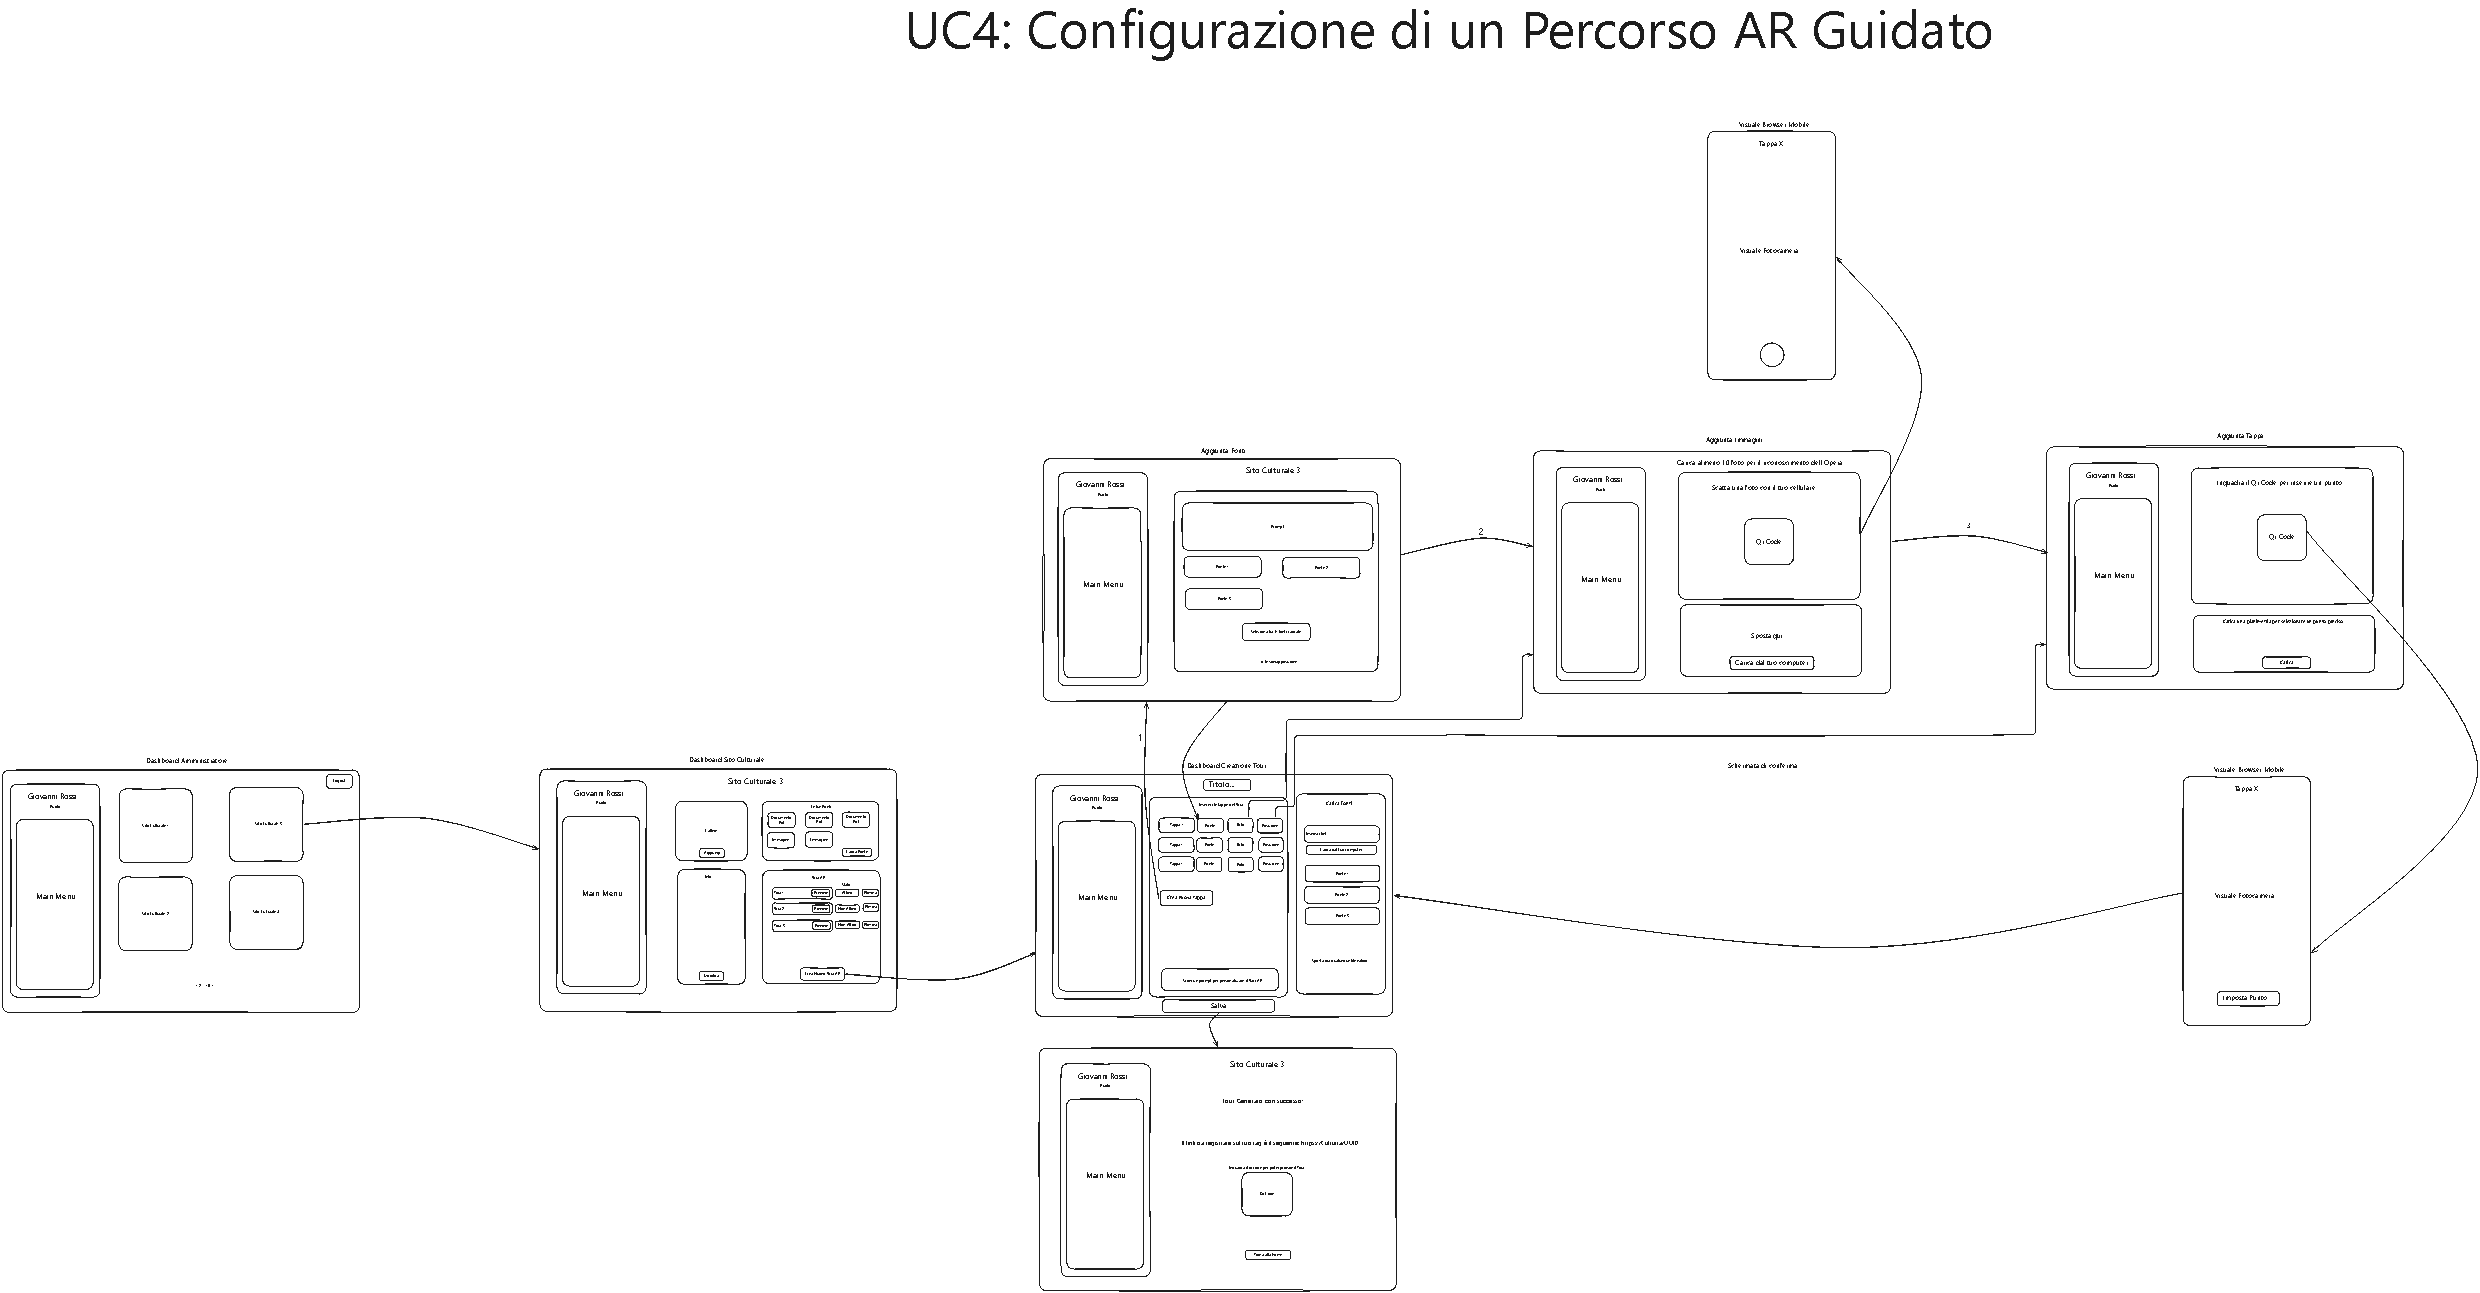
\includegraphics[angle=90, height=0.82\textheight, keepaspectratio]{sketches/UC4_V1_fixed.pdf}
    \caption{Per consultare il PDF originale clicca \href{https://github.com/AntonioWalter/Culturia_IUM/blob/main/docs/allegati/sketches/UC4_V1.pdf}{[QUI]}}
    \label{fig:uc4_v1}
\end{figure}

\newpage
\begin{figure}[H]
    \centering
    \textbf{Use Case 4 - Versione 2} \\[0.5em]
    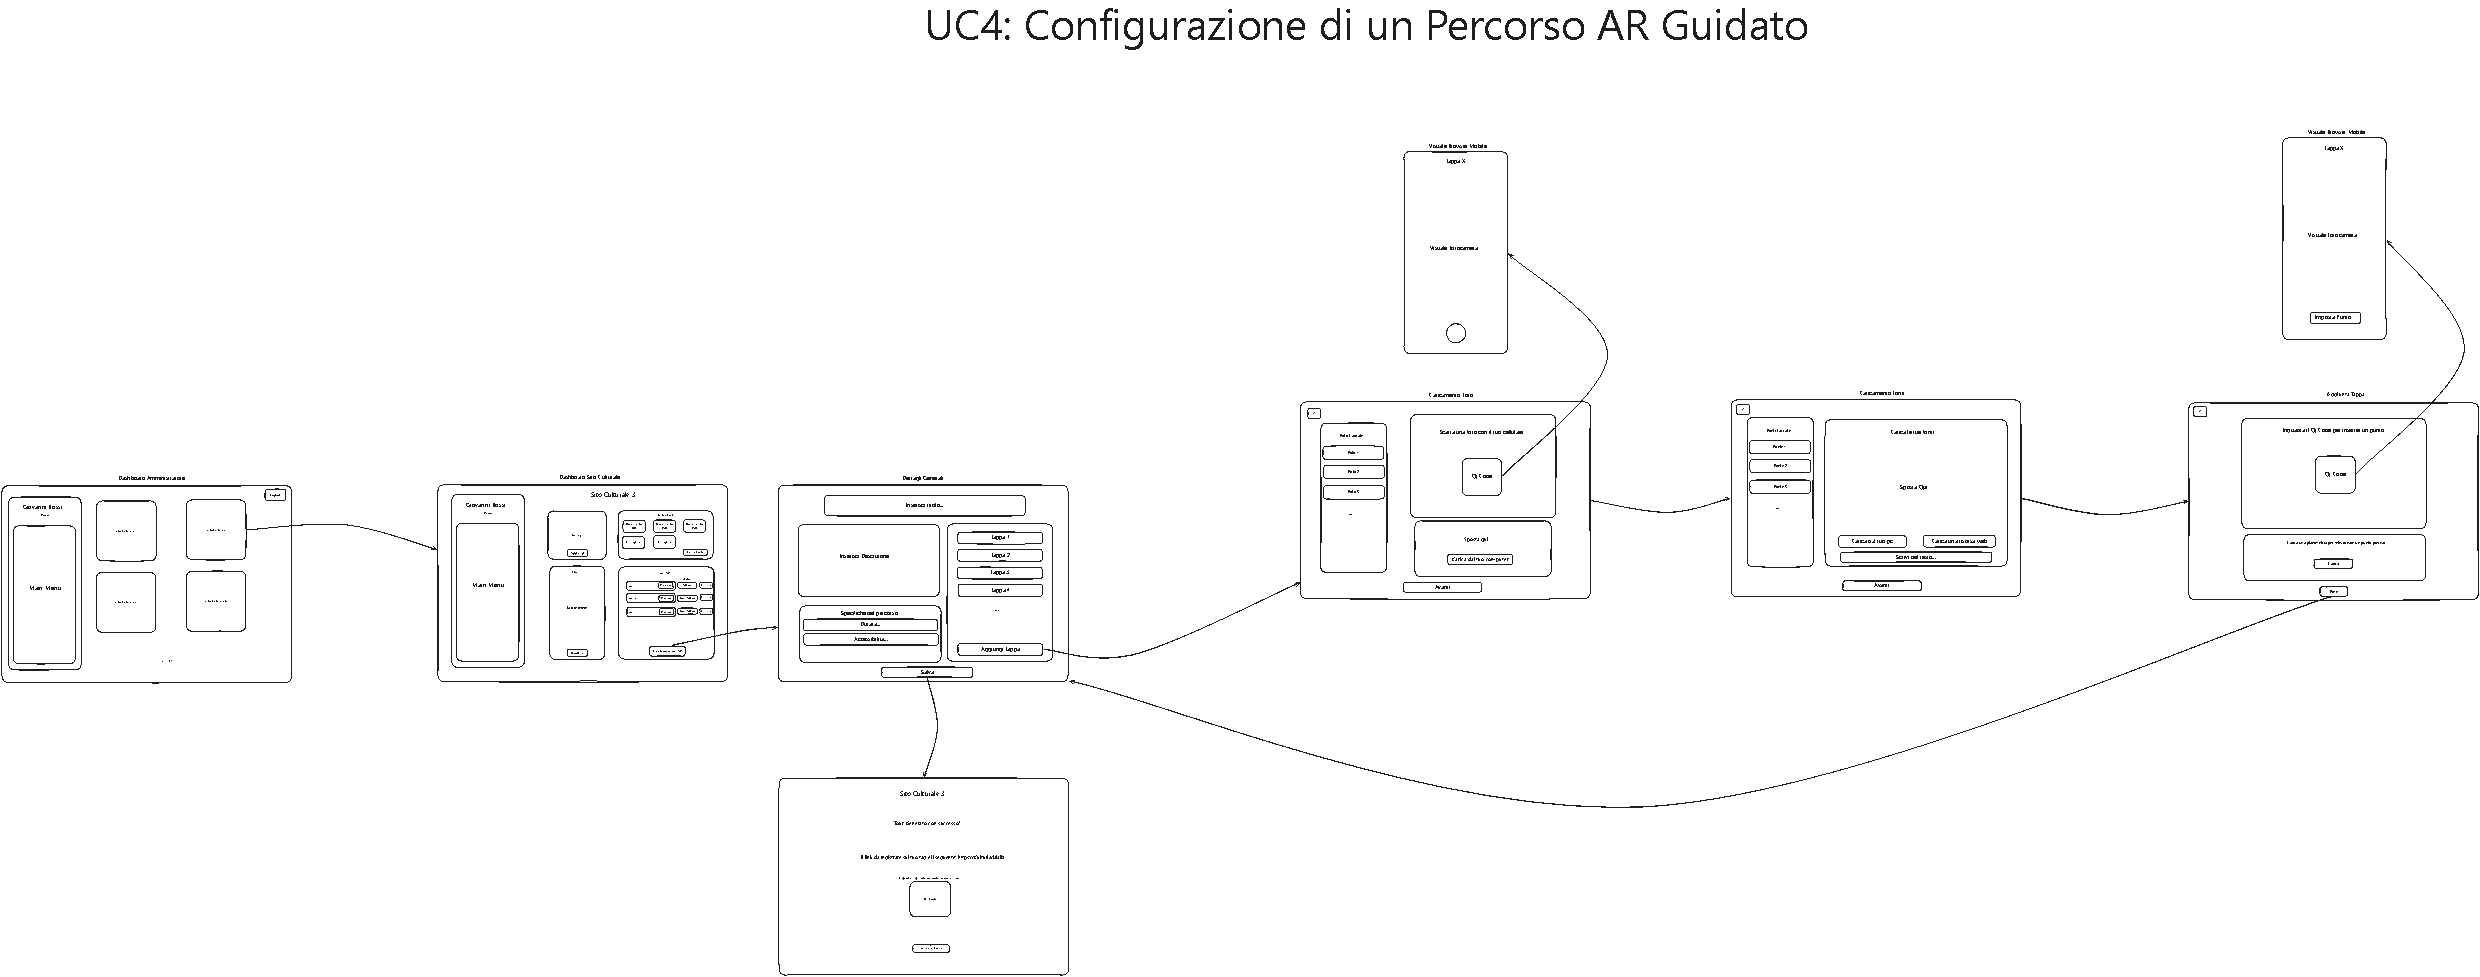
\includegraphics[angle=90, height=0.82\textheight, keepaspectratio]{sketches/UC4_V2_fixed.pdf}
    \caption{Per consultare il PDF originale clicca \href{https://github.com/AntonioWalter/Culturia_IUM/blob/main/docs/allegati/sketches/UC4_V2.pdf}{[QUI]}}
    \label{fig:uc4_v2}
\end{figure}
